\documentclass[10pt]{article}
\usepackage[margin=1in]{geometry}
\usepackage{amsmath,amssymb,bm}
\usepackage{graphicx}
\usepackage{booktabs}
\usepackage{microtype}
\usepackage[hidelinks]{hyperref}
\usepackage[numbers,sort&compress]{natbib}
\usepackage{titlesec}
\usepackage{enumitem}
\linespread{0.94}
\setlist{nosep,leftmargin=*}
\titlespacing*{\section}{0pt}{0.75ex plus 0.2ex}{0.35ex}
\titlespacing*{\subsection}{0pt}{0.55ex plus 0.1ex}{0.25ex}
\titleformat{\section}{\normalsize\bfseries}{\thesection.}{0.4em}{}
\titleformat{\subsection}{\normalsize\bfseries}{\thesubsection.}{0.4em}{}
\setlength{\parindent}{0pt}
\setlength{\parskip}{2pt}
\setlength{\abovedisplayskip}{4pt}
\setlength{\belowdisplayskip}{4pt}
\setlength{\textfloatsep}{7pt}
\setlength{\floatsep}{6pt}
\setlength{\intextsep}{6pt}
\graphicspath{{figures/}}

\newcommand{\dd}{\mathrm{d}}
\newcommand{\cG}{\frac{8\pi G}{c^4}}
\newcommand{\Gobs}{G_{\mu\nu}[g^{\rm obs}]}
\newcommand{\Gbar}{G_{\mu\nu}[g^{\rm bar}]}
\newcommand{\Tmiss}{T^{\rm miss}_{\mu\nu}}

\title{A Residual-of-Residual Test of NFW Geometry in the Missing-Mass Problem}
\author{J. R. Landers}
\date{\vspace{-0.6em}May 2026}

\begin{document}
\maketitle
\vspace{-1.8em}

\begin{abstract}
This short note applies the geometric-residual framework of
\citet{Landers2026Residuals} to the simplest cold-dark-matter baseline: a
pure Navarro-Frenk-White (NFW) halo. The question is not whether cold dark
matter can be embedded in general relativity; it can. The sharper question is
whether the weak-field residual geometry expected from a flat rotation curve is
naturally reproduced by a pure NFW source. A synthetic flat-curve target from
the parent warp-search experiment is fit with NFW, cored/isothermal, and
log-potential residual families. NFW can match the outer flat part when fit
only over the outer galaxy, but then it overpredicts the central residual. When
fit over the full radial range, it loses the expected flat-curve acceleration
slope. In residual language, the remaining ``residual of the residual'' is a
structured correction to the source geometry, not random noise.
\end{abstract}

\section{Question}

The parent paper \citep{Landers2026Residuals} reframes the missing-mass problem
as an inverse problem over spacetime residuals. Instead of asking first which
named theory is correct, it asks which geometric perturbation must be added to
the baryon-predicted metric:
\begin{equation}
g_{\mu\nu}^{\rm trial}
=
g_{\mu\nu}^{\rm bar}
+
h_{\mu\nu}.
\end{equation}
The relativistic residual is
\begin{equation}
\Delta G_{\mu\nu}
:=
\Gobs-\Gbar,
\qquad
\Tmiss
:=
\frac{c^4}{8\pi G}\Delta G_{\mu\nu}.
\end{equation}
If ordinary general relativity is retained, then a dark-matter model is a
candidate stress-energy source for this residual.

For galaxies in the weak-field, nonrelativistic limit,
\begin{equation}
\dd s^2
\simeq
-\left(1+\frac{2\Phi}{c^2}\right)c^2\dd t^2
+
\left(1-\frac{2\Psi}{c^2}\right)\dd\mathbf{x}^2,
\end{equation}
and circular speeds primarily constrain $\Phi$:
\begin{equation}
v^2(r)=r\frac{\dd\Phi}{\dd r}.
\end{equation}
The practical residual used here is therefore
\begin{equation}
\boxed{
\Delta g(r)
=
g_{\rm obs}(r)-g_{\rm bar}(r)
=
\frac{v_{\rm obs}^2(r)-v_{\rm bar}^2(r)}{r}.
}
\end{equation}
In a spherical diagnostic reduction, this residual defines
\begin{equation}
M_{\rm eff}(<r)
=
\frac{r^2\Delta g(r)}{G},
\qquad
\rho_{\rm eff}(r)
=
\frac{1}{4\pi G r^2}
\frac{\dd}{\dd r}
\left[
r^2\Delta g(r)
\right].
\end{equation}

This note tests a narrow scientific claim: after the best pure NFW fit, what
geometry is still missing? Define
\begin{equation}
\boxed{
\epsilon_g(r)
=
\Delta g_{\rm target}(r)
-
\Delta g_{\rm NFW}(r),
}
\end{equation}
and its corresponding effective density proxy
\begin{equation}
\boxed{
\epsilon_\rho(r)
=
\frac{1}{4\pi G r^2}
\frac{\dd}{\dd r}
\left[
r^2\epsilon_g(r)
\right].
}
\end{equation}
This is the residual of the residual: the part of the inferred geometry not
explained by the selected physical source.

\section{NFW in Residual Space}

The NFW density profile \citep{Navarro1996} is
\begin{equation}
\rho_{\rm NFW}(r)
=
\frac{\rho_s}{(r/r_s)(1+r/r_s)^2}.
\end{equation}
With $x=r/r_s$, the enclosed mass is
\begin{equation}
M_{\rm NFW}(<r)
=
4\pi \rho_s r_s^3
\left[
\ln(1+x)-\frac{x}{1+x}
\right].
\end{equation}
The corresponding weak-field residual acceleration is
\begin{equation}
\Delta g_{\rm NFW}(r)
=
\frac{G M_{\rm NFW}(<r)}{r^2}.
\end{equation}
This is a direct source-side prediction for the residual, once the two halo
parameters are fixed.

A flat rotation residual asks for a different shape over the flat part of the
curve:
\begin{equation}
v_{\rm extra}^2\simeq v_f^2
\quad\Rightarrow\quad
\Delta g_{\rm target}(r)
\simeq
\frac{v_f^2}{r},
\qquad
\delta\Phi_{\rm target}
\simeq
v_f^2\log r.
\end{equation}
Thus the expected acceleration slope is
\begin{equation}
\frac{\dd\ln\Delta g_{\rm target}}{\dd\ln r}
\simeq
-1.
\end{equation}
For NFW, writing
\begin{equation}
f(x)=\ln(1+x)-\frac{x}{1+x},
\end{equation}
the local acceleration slope is
\begin{equation}
\boxed{
\frac{\dd\ln\Delta g_{\rm NFW}}{\dd\ln r}
=
\frac{x^2}{(1+x)^2 f(x)}
-
2.
}
\end{equation}
This equals $-1$ only near $x\simeq 2.16$. It remains in the loose flat-curve
band $-1.15<s<-0.85$ only over $1.45\lesssim x\lesssim 3.32$, about 0.36 dex in
radius. NFW can therefore mimic a logarithmic-potential residual over a finite
scale-radius band, but not as a general residual geometry.

\section{Experiment}

The target is the synthetic flat-curve residual from the geometry-first warp
search of \citet{Landers2026Residuals}. The baryonic profile is the same toy
exponential-disk-inspired cumulative mass used there,
\begin{equation}
M_{\rm bar}(<r)
=
M_b\left[
1-e^{-r/R_d}\left(1+\frac{r}{R_d}\right)
\right],
\qquad
g_{\rm bar}(r)=\frac{G M_{\rm bar}(<r)}{r^2}.
\end{equation}
The observed curve is generated by adding a flat-speed component,
\begin{equation}
v_{\rm obs}^2(r)
=
v_{\rm bar}^2(r)
+
\left[
v_f\left(1-e^{-r/r_f}\right)
\right]^2,
\end{equation}
with $v_f=190$ in the toy velocity units and $r_f=4.5$ in the toy radial units.
The resulting target residual rises through the inner galaxy and approaches
$v_f^2/r$ in the outer region.

\begin{figure}[t]
\centering
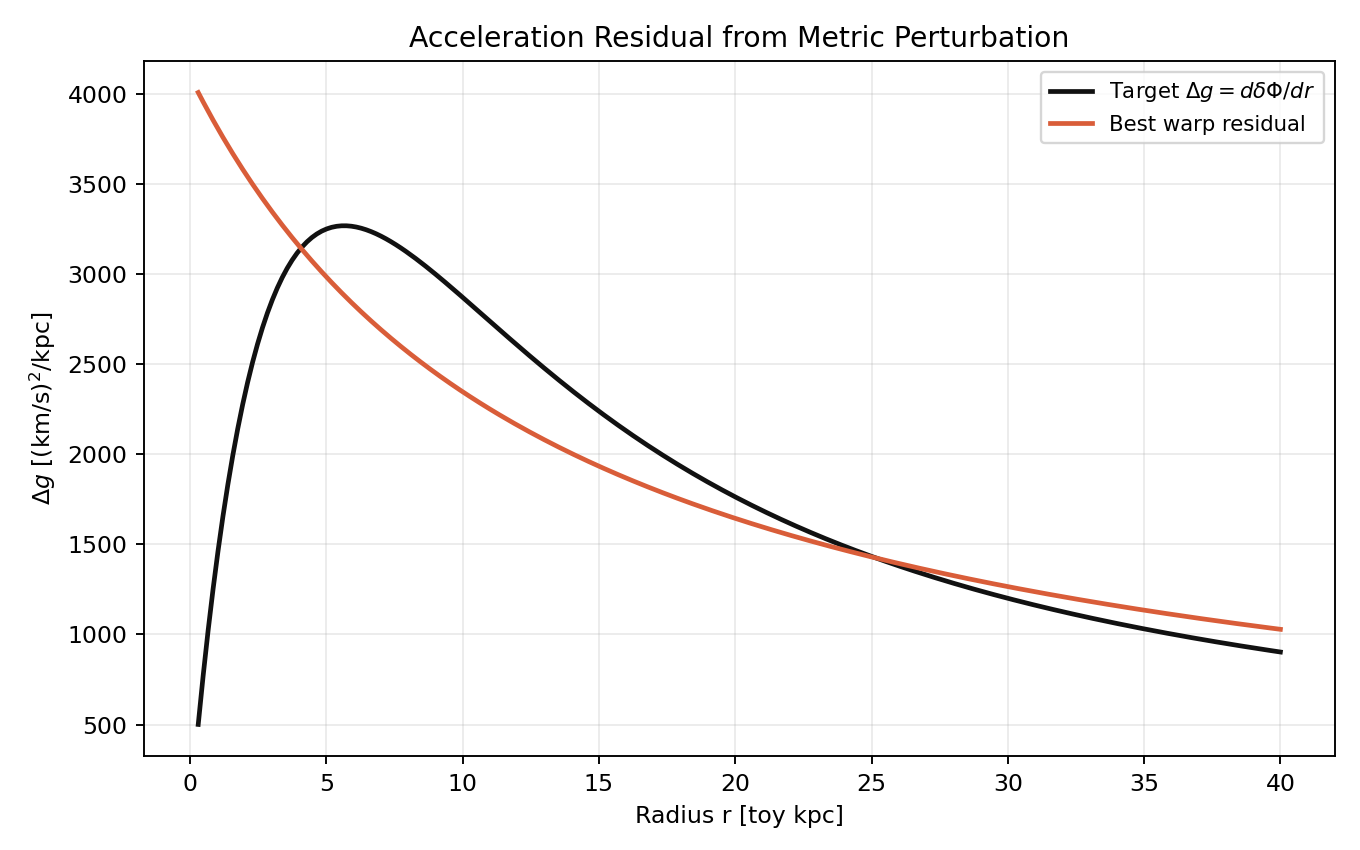
\includegraphics[width=0.66\linewidth]{warp_residual_acceleration.png}
\caption{Target residual inherited from the parent warp search
\citep{Landers2026Residuals}. The synthetic flat-speed component produces an
outer acceleration residual close to $\Delta g\propto 1/r$, equivalent to a
logarithmic potential perturbation over the flat part of the curve.}
\label{fig:target}
\end{figure}

Three families were fit to $\Delta g_{\rm target}$:
\begin{align}
\Delta g_{\rm NFW}(r)
&=
\frac{G M_{\rm NFW}(<r)}{r^2},
\\
\Delta g_{\rm iso}(r)
&=
\frac{v_0^2 r}{r^2+r_c^2},
\\
\Delta g_{\log}(r)
&=
\frac{A}{r+r_0}.
\end{align}
The cored/isothermal profile is included as a control because it is explicitly
designed to approach $\Delta g\propto 1/r$ outside its core. The log-potential
tail is included as a minimal two-parameter warp-like comparison. Fits were
performed over four radial windows: the full $0.3$--$40$ range, $1$--$15$,
$3$--$30$, and $10$--$40$. The key diagnostic is whether a model can match both
the inner transition and the outer flat-curve residual without leaving a
structured $\epsilon_g$.

\begin{table}[t]
\centering
\small
\begin{tabular}{llrrrrr}
\toprule
Model & Fit range & Rel. RMSE & Mean frac. err. & Outer flat. & Outer slope & Near $-1$ frac. \\
\midrule
NFW & 0.3--40 & 0.258 & 0.213 & 0.102 & -0.480 & 0.000 \\
NFW & 3--30 & 0.311 & 0.192 & 0.055 & -0.744 & 0.301 \\
NFW & 10--40 & 0.504 & 0.231 & 0.025 & -0.917 & 0.681 \\
Cored/isothermal & 0.3--40 & 0.031 & 0.020 & 0.028 & -0.868 & 0.699 \\
\bottomrule
\end{tabular}
\caption{Residual-space fits to the synthetic flat-curve target. ``Outer
slope'' is the mean of $\dd\ln\Delta g/\dd\ln r$ over $10\le r\le 40$.
``Near $-1$ frac.'' is the fraction of outer points with slope between $-1.15$
and $-0.85$. The target has mean outer slope $-0.891$ and near-$-1$ fraction
$0.735$.}
\label{tab:fits}
\end{table}

\begin{figure}[t]
\centering
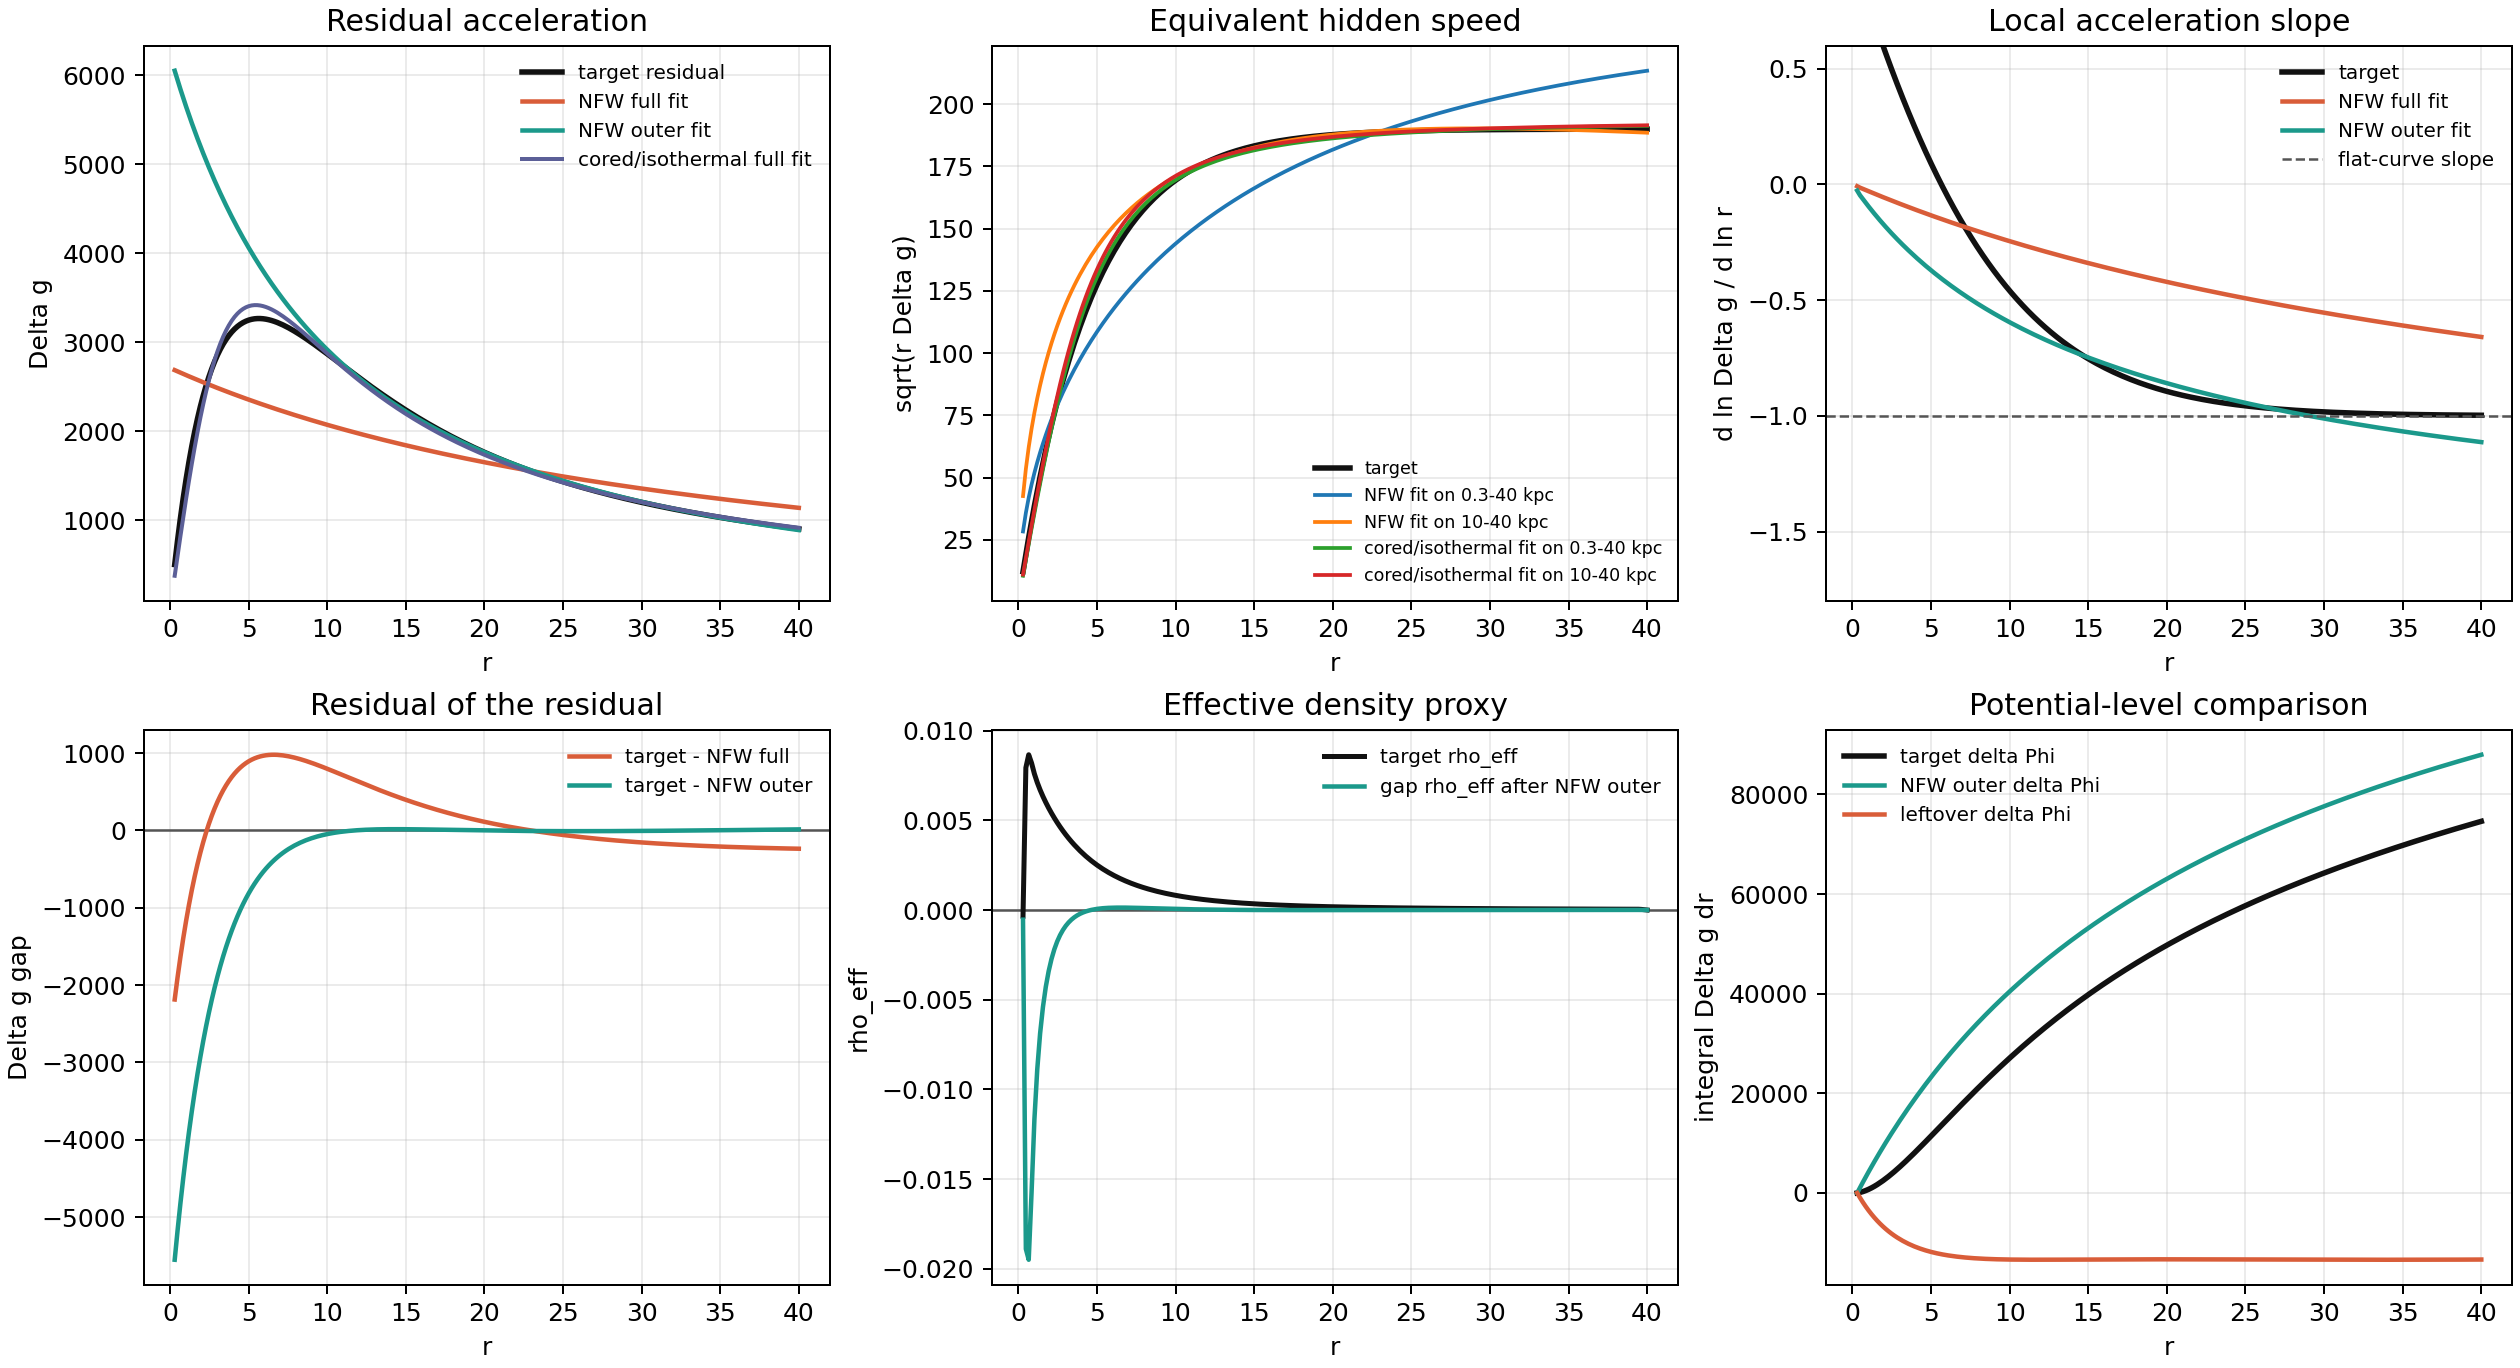
\includegraphics[width=\linewidth]{nfw_residual_of_residual.png}
\caption{Residual-of-residual diagnostic for pure NFW. Top left: the full-range
NFW fit misses the target shape, while the outer-range NFW fit matches the flat
tail but overshoots the inner residual. Top middle and right: the outer NFW fit
recovers the flat hidden speed and near-$-1$ acceleration slope only over the
outer range. Bottom left: the leftover $\epsilon_g=\Delta g_{\rm target}-
\Delta g_{\rm NFW}$ is structured, not noise. Bottom middle: interpreted as an
effective source correction, the leftover after the outer NFW fit is strongly
negative in the inner region. Bottom right: the potential-level comparison
shows that the outer NFW fit accumulates too much central potential before
tracking the flat-curve tail.}
\label{fig:nfw}
\end{figure}

\section{Results}

The experiment produces two complementary failures.

First, a full-range NFW fit spreads its scale radius outward:
\begin{equation}
{\rm mass\ scale}=257.84,
\qquad
r_s=45.23.
\end{equation}
This lowers the central overshoot, but the outer acceleration slope becomes too
shallow. Over $10\le r\le 40$, the mean NFW slope is $-0.480$, whereas the
target slope is $-0.891$. None of the outer points are in the loose flat-curve
slope band.

Second, an outer-only NFW fit chooses
\begin{equation}
{\rm mass\ scale}=52.29,
\qquad
r_s=13.43.
\end{equation}
This is the fit NFW wants if the task is only to match the flat tail. It gives
outer flatness $0.025$ and mean outer slope $-0.917$, almost exactly the
expected logarithmic-potential residual. But the full relative RMSE worsens to
$0.504$ because the same NFW halo overpredicts the central residual by a large
amount. In the residual-of-residual field, this appears as a negative inner
source correction:
\begin{equation}
\epsilon_g(r)<0
\quad
\text{through most of the inner region.}
\end{equation}
The corresponding $\epsilon_\rho$ is also negative over the central correction
region. This is not a physical negative matter claim by itself; it is a
diagnostic statement: after pure NFW is forced to explain the outer geometry,
the remaining geometry asks for removal or redistribution of central source
structure.

The cored/isothermal control demonstrates that the target is not hard to fit in
residual space. Its full-range fit gives relative RMSE $0.031$ and mean
fractional error $0.020$, with mean outer slope $-0.868$. This is expected:
\begin{equation}
\Delta g_{\rm iso}(r)
=
\frac{v_0^2 r}{r^2+r_c^2}
\longrightarrow
\frac{v_0^2}{r}
\quad
(r\gg r_c).
\end{equation}
The control is not presented as the correct theory. It is a shape test showing
that the residual target prefers an extended, cored, nearly logarithmic
potential structure over this radial range.

\section{Interpretation}

This result is the cusp/core tension expressed in the language of residual
geometry \citep{deBlok2010}. Pure NFW is a valid stress-energy source inside
general relativity, but its residual acceleration shape is not freely
logarithmic. It has three characteristic regimes:
\begin{align}
r\ll r_s &: \rho\sim r^{-1},\quad M(<r)\sim r^2,\quad \Delta g\sim {\rm const},\\
r\sim r_s &: \Delta g \text{ can mimic } 1/r \text{ over a finite band},\\
r\gg r_s &: \rho\sim r^{-3},\quad M(<r)\sim \log r,\quad
\Delta g\sim \frac{\log r}{r^2}.
\end{align}
Therefore the NFW explanation of a flat rotation residual requires the observed
flat region to align with the halo's scale-radius band. If the same profile is
required to fit the inner transition, the alignment is lost.

The residual-of-residual object makes this failure useful rather than merely
negative. A random residual would suggest noise or an underfit. A structured
inner negative correction suggests a specific missing element: core formation,
baryonic feedback, a non-NFW phase-space distribution, self-interactions,
wave-like pressure, a modified source decomposition, or some systematic error
in the target construction. The present experiment does not choose among those
possibilities. It only says what the geometry asks for after pure NFW has done
its best.

\section{Limitations and Next Tests}

This is a synthetic weak-field experiment, not a real galaxy fit. The inversion
uses a spherical effective-density proxy, not a disk model. The target is built
from a chosen flat-speed component rather than from SPARC data
\citep{Lelli2016}. No cosmological halo-concentration prior is imposed. No
lensing observable is fit. The diagnostic is therefore a controlled shape test,
not evidence against cold dark matter as a full theory.

The immediate next step is to repeat the same residual-of-residual calculation
on real rotation curves with disk geometry:
\begin{equation}
\epsilon_g(r)
=
\Delta g_{\rm inferred}(r)
-
\Delta g_{\rm candidate}(r),
\end{equation}
then classify $\epsilon_g$ and $\epsilon_\rho$ across galaxies. If the leftover
geometry clusters into repeated families, those families become stronger
targets for physics: feedback-generated cores, self-interacting halos,
ultralight scalar cores, warm-dark-matter phase-space limits, baryonic
systematics, or modified-gravity terms.

\section{Compact Conclusion}

In the parent geometric-residual framework, the question is not just whether a
dark-matter candidate exists. It is whether its stress-energy produces the
observed residual geometry:
\begin{equation}
\Delta G_{\mu\nu}
\stackrel{?}{=}
\cG T^{\rm candidate}_{\mu\nu}.
\end{equation}
For the synthetic flat-curve target tested here, pure NFW/CDM gives a clear
answer: it can match the outer logarithmic-potential residual, or it can reduce
the inner overshoot, but it does not naturally do both with one profile. The
leftover field is structured and interpretable. That is the value of the
residual-of-residual test: it turns a familiar model mismatch into an explicit
geometric object that can be compared across candidate physics.

\begingroup\small
\begin{thebibliography}{9}

\bibitem[Landers(2026)]{Landers2026Residuals}
Landers, J. R. (2026).
Geometric residuals and weak-field warp search in the missing-mass problem.
Unpublished manuscript, May 2026.

\bibitem[Navarro et~al.(1996)]{Navarro1996}
Navarro, J. F., Frenk, C. S., \& White, S. D. M. (1996).
The structure of cold dark matter halos.
\emph{The Astrophysical Journal}, 462, 563--575.
\href{https://doi.org/10.1086/177173}{doi:10.1086/177173}.

\bibitem[Rubin et~al.(1980)]{Rubin1980}
Rubin, V. C., Ford, W. K., Jr., \& Thonnard, N. (1980).
Rotational properties of 21 Sc galaxies with a large range of luminosities and radii.
\emph{The Astrophysical Journal}, 238, 471--487.
\href{https://doi.org/10.1086/158003}{doi:10.1086/158003}.

\bibitem[Lelli et~al.(2016)]{Lelli2016}
Lelli, F., McGaugh, S. S., \& Schombert, J. M. (2016).
SPARC: Mass models for 175 disk galaxies with Spitzer photometry and accurate rotation curves.
\emph{The Astronomical Journal}, 152, 157.
\href{https://doi.org/10.3847/0004-6256/152/6/157}{doi:10.3847/0004-6256/152/6/157}.

\bibitem[McGaugh et~al.(2016)]{McGaugh2016}
McGaugh, S. S., Lelli, F., \& Schombert, J. M. (2016).
The radial acceleration relation in rotationally supported galaxies.
\emph{Physical Review Letters}, 117, 201101.
\href{https://doi.org/10.1103/PhysRevLett.117.201101}{doi:10.1103/PhysRevLett.117.201101}.

\bibitem[de Blok(2010)]{deBlok2010}
de Blok, W. J. G. (2010).
The core-cusp problem.
\emph{Advances in Astronomy}, 2010, 789293.
\href{https://doi.org/10.1155/2010/789293}{doi:10.1155/2010/789293}.

\bibitem[Bertone \& Hooper(2018)]{Bertone2018}
Bertone, G., \& Hooper, D. (2018).
History of dark matter.
\emph{Reviews of Modern Physics}, 90, 045002.
\href{https://doi.org/10.1103/RevModPhys.90.045002}{doi:10.1103/RevModPhys.90.045002}.

\end{thebibliography}
\endgroup

\end{document}
